A lot of tools are available on the Internet to manage the creation of Graphical User Interfaces (GUI). These kinds of software provide classes, function and usually a ``designer" mode to facilitate the creation of an interface. The most famous I discovered on the Internet are Qt, WxWidget, GTK+, FLTK, FOX. If necessary, I would have been ready to learn any programming language to achieve my project, luckily for me most of the available tools are develop in C++. During this year of Computing Science master at Imperial College of London I learned a lot on the C++ languages, firstly through lectures and lab session, and also through my group project. Hence, it was really time saving for me not to look for other tools. 

\newline \vspace{5mm}

In order to be sure to use a widget library that will suit me I have decided to compare the provided one before picking one. I couldn't compare all of them, so I have decided to focus on Qt, WxWidget GTK+.I looked across the Internet to get some testimonies about the different tools and I tried to distinguish them following several criteria - see grid below. According to these criteria and considering that Qt is highly recommended for beginners, I have finally decided to use Qt for this project.

\begin{figure}[ht]
\centering
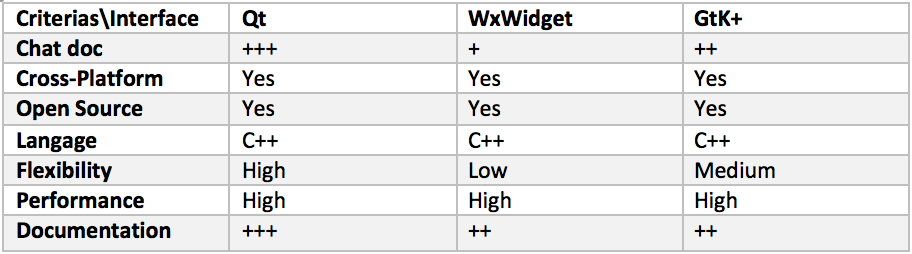
\includegraphics[width = 0.99\hsize]{./figures/comparison}
\caption{Qt, WxWidget, GTK+ comparison table}
\end{figure}
 

In order to get used to Qt, which was new to me, I have decided to complete Openclassroom tutorials [6]. Those tutorials have helped me to install QtCreator and to get familiar with Qt beginning with some basic exercices.